\documentclass[a4paper]{scrartcl}
\usepackage[english]{babel}
\usepackage[top=2cm,bottom=3cm,left=2.5cm,right=2.5cm]{geometry}
\usepackage[colorlinks=true, allcolors=black]{hyperref}
\usepackage{wrapfig} %문단 내 이미지 삽입
\usepackage{graphicx} %색상
\usepackage{overpic}
\usepackage[normalem]{ulem}%취소선
\usepackage{array} %표
\usepackage{mdframed, tcolorbox} %글상자
\usepackage[yyyymmdd]{datetime}
	\renewcommand{\dateseparator}{--}
\usepackage{amsmath, amsfonts, amssymb, bm} %수식
	\DeclareMathOperator{\arccsc}{arccsc}
	\DeclareMathOperator{\arcsec}{arcsec}
	\DeclareMathOperator{\arccot}{arccot}
	\DeclareMathOperator{\csch}{csch}
	\DeclareMathOperator{\sech}{sech}
	\DeclareMathOperator{\arcsinh}{arcsinh}
	\DeclareMathOperator{\arccosh}{arccosh}
	\DeclareMathOperator{\arctanh}{arctanh}
	\DeclareMathOperator{\arccsch}{arccsch}
	\DeclareMathOperator{\arcsech}{arcsech}
	\DeclareMathOperator{\arccoth}{arccoth}
	
	\DeclareMathOperator{\meter}{m}
	\DeclareMathOperator{\cm}{cm}
	\DeclareMathOperator{\mm}{mm}
	\DeclareMathOperator{\mum}{\mu m}
	\DeclareMathOperator{\newton}{N}
	\DeclareMathOperator{\kn}{kN}
	\DeclareMathOperator{\kgf}{kgf}
	\DeclareMathOperator{\pa}{Pa}
	\DeclareMathOperator{\kpa}{kPa}
	\DeclareMathOperator{\mpa}{MPa}
	\DeclareMathOperator{\gpa}{GPa}
	\DeclareMathOperator{\knpm}{kN/m}
	\DeclareMathOperator{\kph}{km/h}
	\DeclareMathOperator{\mps}{m/s}
	\DeclareMathOperator{\tkph}{kph}
	\DeclareMathOperator{\tmps}{mps}
	\DeclareMathOperator{\mpss}{m/s^2}
	\DeclareMathOperator{\dgr}{\!^\circ}
	\DeclareMathOperator{\cel}{\!^\circ C}
	\DeclareMathOperator{\kg}{kg}
	\DeclareMathOperator{\kgpcm}{kg/m^3}
	\DeclareMathOperator{\nm}{N\cdot m}
	\DeclareMathOperator{\knm}{kN\cdot m}
	\DeclareMathOperator{\kw}{kW}
	\DeclareMathOperator{\kwh}{kWh}
	\DeclareMathOperator{\mmhg}{mmHg}
	\DeclareMathOperator{\snd}{s}
	\DeclareMathOperator{\joule}{J}
\usepackage{polynom} %나눗셈 필산
\usepackage{cancel} %수식 약분선
\usepackage{titlesec} %섹션 이름 변경
	\titlespacing*{\section}{3mm}{0mm}{1mm}
	\titleformat{\section}{\bfseries\large}{}{0ex}{}
\usepackage{kotex} %한글

\newcommand{\prob}[2]{\section{#1}\begin{mdframed}#2\end{mdframed}}

\newlength{\picwidth}
\newcommand{\probpic}[4]{
	\setlength{\picwidth}{145mm}\addtolength{\picwidth}{-#3}\section{#1}\begin{mdframed}\begin{tabular}{m{#3}m{\picwidth}}
	\includegraphics[width = #3]{#2} & #4\end{tabular}\end{mdframed}
	}
	
\newcommand{\asw}[2]{
	\begin{flushright}
		#1\quad$\blacktriangleleft$\quad#2
	\end{flushright}
	}
	
\newcommand{\aswtag}[1]{
	\quad\blacktriangleleft\quad#1
	}

\title{\vspace{100pt}\Huge{해설}}
\author{
	구조역학(박성훈 교수님) 2025-2 기말고사\\[10pt]
	시험 실시 : 2025-10-20 16:30-19:30(180분)\\[110pt]
	}
\date{\today}

\begin{document}
	
\renewcommand*{\titlepagestyle}{empty}
\maketitle

\vspace{60pt}

\begin{center}
	\includegraphics[width=0.45\textwidth]{SSU symbol KR-EN.jpg}
\end{center}

\newpage\setcounter{page}{1}

\probpic{Question 1 | Prob. 9.100}{img/q1.png}{55mm}{For the uniform cantilever beam and loading shown, determine the slope and deflection at ($a$) point $B$, ($b$) point $C$. Use the momnet-area method to solve this problem. (부호 또는 화살표를 통해 처짐과 처짐각의 방향을 명확히 표시하시오.)}

\noindent\includegraphics{img/q1-1.png}
In portion $AB$,
\begin{align*}
	&A_m = \frac{1}{3}\cdot \frac{wL^2}{8}\cdot \frac{L}{2} = \frac{wL^3}{48},\quad \bar{x} = \bar{x}_0 = \frac{3}{4}\cdot\frac{L}{2} = \frac{3L}{8}\\
	&\theta_{B/A} = \theta_B = -\frac{A_m}{EI} = -\frac{wL^3}{48EI}\\
	&t_{B/A} = y_B = -\frac{A_m\bar{x}}{EI} = -\frac{wL^4}{128EI}
\end{align*}
\asw{$\theta_B = -\cfrac{wL^3}{48EI}\;;\;y_B = -\cfrac{wL^4}{128EI}$}{($a$)}
In portion $AC$,
\begin{align*}
	&\theta_{C/A} = \theta_C = -\frac{A_m}{EI} = -\frac{wL^3}{48EI}\\
	&y_C = y_B + \theta_B\times\frac{L}{2} = -\frac{7wL^4}{384EI}
\end{align*}
\asw{$\theta_C = -\cfrac{wL^3}{48EI}\;;\;y_C = -\cfrac{7wL^4}{384EI}$}{($b$)}

\newpage

\probpic{Question 2 | Prob. 10.13}{img/q2.png}{45mm}{Determine ($a$) the critical load for the brass strut, ($b$) the dimension $d$ for which the aluminum strut will have the same critical load, ($c$) the weight of the aluminum strut as a percent of the weight of the brass strut.}

\begin{align*}
	&P_\text{cr} = \frac{\pi^2 E_bI_1}{L^2} = \frac{\pi^2(120\times10^9)(\frac{1}{12}\cdot 0.02^4)}{1.1^2}\newton = 13050.71656\newton = 13.05\kn \quad\blacktriangleleft\quad(a)\\
	&P_\text{cr} = \frac{\pi^2E_aI_2}{L^2} = \frac{\pi^2E_ad^4}{12L^2}\quad\Rightarrow\quad d = \left(\frac{12P_\text{cr}L^2}{\pi^2E_a}\right)^{\frac{1}{4}} = 0.0228849937\meter = 22.88\mm \quad\blacktriangleleft\quad(b)\\
	&\frac{m_a}{m_b} = \frac{\rho_a d^2 L}{\rho_b (0.02\meter)^2 L} = \frac{\rho_a d^2}{\rho_b (0.02\meter)^2} = \frac{(2710)(0.228849937)^2}{(8740)(0.02)^2} = 40.60\%\quad\blacktriangleleft\quad(c)
\end{align*}

\newpage

\probpic{Question 3 | variation of Prob. 10.35}{img/q3.png}{45mm}{An axial load $P = 15\kn$ is applied at point $D$ that is $6\mm$ from the geomatric axis of the square aluminum bar $BC$. Using $70\gpa$. determine ($a$) the horizontal deflection of end $C$, ($b$) the corresponding maximum stress in the column.}

\begin{align*}
	&I = \frac{1}{12}(0.03)^4\meter^4 = 6.75\times10^{-8}\meter^4,\quad L_e = 2L = 1.2\meter\\
	&\text{let}\quad H = \sec\left({\frac{L_e}{2}\sqrt{\frac{P}{EI}}}\right) = \sec\left({\frac{1.2}{2}\sqrt{\frac{15\times10^3}{(70\times10^9)(6.75\times10^{-8})}}}\right) = 2.079167354\\
	&y_\text{max} = e(H-1) = 4.32\mm\quad\blacktriangleleft\quad(a)\\
	&\frac{ec}{r^2} = \frac{ecA}{I} = \frac{(0.004)(0.015)(0.03^2)}{6.75\times10^{-8}} = 0.8\\
	&\sigma_\text{max} = \frac{P}{A}\left(1 + \frac{ec}{r^2}\cdot H\right) = 44.39\mpa\quad\blacktriangleleft\quad(b)
\end{align*}

\newpage

\probpic{Question 4 | variation of Prob. 3.36}{img/q4.png}{65mm}{The torques shown are exerted on pulleys $A$ and $B$. Knowing that the shafts are solid and made of steel ($G = 73\gpa$), determine the strain energy of this system.}

\begin{align*}
	&T_{AB} = T_A = 300\nm,\quad T_{BC} = T_A + T_B = 1000\nm\\
	&J_{AB} = \frac{\pi}{2}(0.015^4)\meter^4 = 7.952156404\times10^{-8}\meter^4\\
	&J_{BC} = \frac{\pi}{2}(0.023^4)\meter^4 = 4.395732149\times10^{-7}\meter^4\\
	&U_\text{tot}= \frac{T_{AB}^2L_{AB}}{2GJ_{AB}} + \frac{T_{BC}^2L_{BC}}{2GJ_{BC}} = 18.66\joule\quad\blacktriangleleft
\end{align*}

\newpage

\probpic{Question 5 | variation of Prob. 11.45}{img/q5.png}{55mm}{The 50-kg collar $D$ is released from rest in the position shown and is stopped by a plate attached at end $C$ of the vertical rod $ABC$. Knowing that $E = 200\gpa$ and the maximum normal stress is $250\mpa$ for both portions of the rod, determine the maximum height $h_m$.}

\begin{align*}
	&P_m = \sigma_m A_{BC} = (250\mpa)(\pi\cdot15^2\mm^2) = 176714.5868\newton\\
	&U_m = \frac{P_m^2L_{AB}}{2EA_{AB}} + \frac{P_m^2L_{BC}}{2EA_{BC}} = 289.9223689\joule\\
	&U_m = \frac{1}{2}P_m\delta_m\quad\Rightarrow\quad \delta_m = \frac{2U_m}{P_m} = 3.28125\mm\\
	&U_m = mg(h_m + \delta_m)\quad\Rightarrow\quad h_m = \frac{U_m}{mg} - \delta_m = 0.587793916\meter = 587.79\mm \quad\blacktriangleleft
\end{align*}
	
\end{document}